\documentclass[a4paper,10pt,twocolumn,english]{article}

% ============================================================================
% Packages
% ============================================================================

\usepackage{babel}
\usepackage[utf8]{inputenc}
\usepackage[T1]{fontenc}
\usepackage{lmodern}
\usepackage{amsmath,amssymb,amsthm,mathtools}
\usepackage{graphicx}
\usepackage{booktabs}
\usepackage{array}
\usepackage{tabularx}
\usepackage{longtable}
\usepackage{listings}
\usepackage{xcolor}
\usepackage{hyperref}
\usepackage{url}
\makeatletter
\g@addto@macro\UrlBreaks{\do\/\do\.\do\_\do\-\do\*}
\makeatother
\Urlmuskip=0mu\relax
\usepackage{enumitem}
\usepackage{microtype}
\usepackage{cleveref}
\usepackage[font=small,labelfont=bf]{caption}
\usepackage{float}
\usepackage{tikz}
\usetikzlibrary{positioning,calc,arrows.meta}

% TikZ figure styles
\tikzset{
  figfont/.style={font=\scriptsize\sffamily},
  figbox/.style={draw, rounded corners=2pt, align=center, inner sep=4pt},
  figboxgray/.style={figbox, fill=gray!10},
  figsubbox/.style={figbox, fill=white},
  figsubboxgray/.style={figbox, fill=gray!5},
  figarrow/.style={-{Stealth[length=2mm]}, thick},
  figarrowstrong/.style={figarrow, line width=0.6pt},
}

% Reduce space between section number and title, prevent hyphenation in headings
\makeatletter
\renewcommand{\@seccntformat}[1]{\csname the#1\endcsname\hspace{0.5em}}
\renewcommand{\section}{\@startsection{section}{1}{\z@}%
  {-3.5ex \@plus -1ex \@minus -.2ex}%
  {2.3ex}%
  {\raggedright\normalfont\large\bfseries}}
\renewcommand{\subsection}{\@startsection{subsection}{2}{\z@}%
  {-3.25ex \@plus -1ex \@minus -.2ex}%
  {1.5ex}%
  {\raggedright\normalfont\normalsize\bfseries}}
\renewcommand{\subsubsection}{\@startsection{subsubsection}{3}{\z@}%
  {-3.25ex \@plus -1ex \@minus -.2ex}%
  {1.5ex}%
  {\raggedright\normalfont\small\bfseries}}
\makeatother

% ============================================================================
% Typography improvements
% ============================================================================

\raggedbottom                           % Consistent local spacing
\widowpenalty=10000                     % Prevent widows (single lines at top)
\clubpenalty=10000                      % Prevent orphans (single lines at bottom)
\displaywidowpenalty=10000              % Prevent widows after display math
\predisplaypenalty=50                   % Discourage break before display math
\postdisplaypenalty=50                  % Discourage break after display math
\setlength{\emergencystretch}{2em}      % Reduce overfull lines in narrow columns
\setlength{\columnsep}{16pt}            % Slightly wider gutter for two-column reading
\setlength{\parskip}{0pt plus 1pt}      % Flexible paragraph spacing
\setlength{\floatsep}{10pt plus 2pt minus 2pt}
\setlength{\textfloatsep}{12pt plus 2pt minus 2pt}
\setlength{\intextsep}{10pt plus 2pt minus 2pt}
\setlength{\tabcolsep}{4pt}
\renewcommand{\arraystretch}{1.08}
\renewcommand{\topfraction}{0.85}       % Allow more floats at top
\renewcommand{\bottomfraction}{0.85}    % Allow more floats at bottom
\renewcommand{\textfraction}{0.10}      % Require less text on float pages
\renewcommand{\floatpagefraction}{0.7}  % Fuller float pages
\setcounter{topnumber}{2}
\setcounter{bottomnumber}{1}
\setcounter{totalnumber}{3}
\setlist[itemize]{leftmargin=*, itemsep=2pt, topsep=3pt}
\setlist[enumerate]{leftmargin=*, itemsep=2pt, topsep=3pt}
\setlist[description]{leftmargin=0pt, labelindent=0pt, itemsep=2pt, topsep=3pt}

% ============================================================================
% Numbering by section
% ============================================================================

\makeatletter
\@addtoreset{figure}{section}
\renewcommand{\thefigure}{\thesection.\arabic{figure}}
\@addtoreset{table}{section}
\renewcommand{\thetable}{\thesection.\arabic{table}}
\makeatother
\numberwithin{equation}{section}

% ============================================================================
% Theorem environments
% ============================================================================

\newtheoremstyle{paperplain}%
{3pt}{3pt}{\itshape\raggedright}{}{\bfseries}{}{0pt}%
{\thmname{#1}\thmnumber{ #2}\thmnote{. #3}.\hfill\break}
\newtheoremstyle{paperdef}%
{3pt}{3pt}{\normalfont\raggedright}{}{\bfseries}{}{0pt}%
{\thmname{#1}\thmnumber{ #2}\thmnote{. #3}.\hfill\break}
\newtheoremstyle{paperremark}%
{3pt}{3pt}{\normalfont\raggedright}{}{\itshape}{}{0pt}%
{\thmname{#1}\thmnumber{ #2}\thmnote{. #3}.\hfill\break}

\theoremstyle{paperdef}
\newtheorem{definition}{Definition}[section]

\theoremstyle{paperplain}
\newtheorem{theorem}[definition]{Theorem}
\newtheorem{lemma}[definition]{Lemma}
\newtheorem{proposition}[definition]{Proposition}
\newtheorem{corollary}[definition]{Corollary}

\theoremstyle{paperdef}
\newtheorem{example}[definition]{Example}
\newtheorem{assumption}{Assumption Block}[section]

\theoremstyle{paperremark}
\newtheorem{remark}[definition]{Remark}

\theoremstyle{paperdef}
\newtheorem{assumptions}[assumption]{Assumption Block}

% ============================================================================
% Custom commands
% ============================================================================

\newcolumntype{L}[1]{>{\raggedright\arraybackslash}p{#1}}
\newcommand{\thead}[1]{\textbf{\raisebox{0pt}[2.2ex][0.8ex]{#1}}}

\newcommand{\Hbyz}{\ensuremath{H_{\mathrm{byz}}}}
\newcommand{\Obssafe}{\ensuremath{\mathsf{Obs}_{\mathrm{safe}}^{\mathrm{byz}}}}
\newcommand{\Eqsafe}{\ensuremath{\mathsf{Eq}_{\mathrm{safe}}^{\mathrm{byz}}}}
\newcommand{\Ebyz}{\ensuremath{\mathcal{E}_{\mathrm{byz}}}}
\newcommand{\ByzSafe}{\ensuremath{\mathsf{ByzSafe}}}
\newcommand{\ByzChar}{\ensuremath{\mathsf{ByzChar}}}
\newcommand{\Coherent}{\ensuremath{\mathsf{Coherent}}}
\newcommand{\Harmony}{\ensuremath{\mathsf{Harmony}}}
\newcommand{\Admissible}{\ensuremath{\mathsf{Admissible}}}
\newcommand{\EnvelopeRel}{\ensuremath{\mathsf{EnvelopeRel}}}
\newcommand{\EnvelopeExact}{\ensuremath{\mathsf{EnvelopeExact}}}
\newcommand{\EnvelopeOK}{\ensuremath{\mathsf{EnvelopeOK}}}
\newcommand{\ConfigEquiv}{\ensuremath{\mathsf{ConfigEquiv}}}
\newcommand{\ExchangeEq}{\ensuremath{\mathsf{ExchangeEq}}}
\newcommand{\Obs}{\ensuremath{\mathsf{Obs}}}
\newcommand{\ProjStep}[2]{\ensuremath{\mathsf{ProjStep}_{#2}(#1)}}
\newcommand{\LocStep}[2]{\ensuremath{\mathsf{LocStep}_{#2}(#1)}}
\newcommand{\ProjLink}[1]{\ensuremath{\mathsf{ProjLinkStep}(#1)}}
\newcommand{\LocLink}[1]{\ensuremath{\mathsf{LocLinkStep}(#1)}}
\newcommand{\ProjDelegate}[1]{\ensuremath{\mathsf{ProjDelegateStep}(#1)}}
\newcommand{\LocDelegate}[1]{\ensuremath{\mathsf{LocDelegateStep}(#1)}}
\newcommand{\JointActive}[1]{\ensuremath{\mathsf{JointRealizable}_{\mathsf{active}}(#1)}}
\newcommand{\EqsafeConformance}{\ensuremath{\mathsf{EqsafeConformance}}}
\newcommand{\VMAdheres}{\ensuremath{\mathsf{VMAdheres}}}
\newcommand{\HasProfileCapabilities}{\ensuremath{\mathsf{HasProfileCapabilities}}}
\newcommand{\wf}{\ensuremath{\mathsf{wf}}}
\newcommand{\envG}{\ensuremath{\mathsf{envG}}}
\newcommand{\envD}{\ensuremath{\mathsf{envD}}}
\newcommand{\pathref}[1]{\texttt{#1}}
\newcommand{\eqnote}[1]{\par\noindent\textit{#1.}\par\vspace{-2pt}}
\newcommand{\ABHStack}{Theorems~\ref{thm:harmony}, \ref{thm:erasure}, \ref{thm:delegation}, \ref{thm:minimality}, \ref{thm:conservation}, \ref{thm:envelope}, \ref{thm:normalization}, and~\ref{thm:adequacy}}

\newenvironment{citelist}{%
  \begin{list}{}{%
    \setlength{\leftmargin}{1.25em}%
    \setlength{\itemindent}{-1.25em}%
    \setlength{\itemsep}{2pt}%
    \setlength{\parsep}{0pt}%
    \setlength{\topsep}{3pt}}%
}{\end{list}}

\lstset{
  basicstyle=\ttfamily\footnotesize,
  keywordstyle=\color{blue},
  commentstyle=\color{gray},
  stringstyle=\color{red},
  breaklines=true,
  frame=leftline,
  rulecolor=\color{black!10},
  framerule=3pt,
  framesep=1em,
  columns=fullflexible,
  aboveskip=5pt,
  belowskip=5pt,
  xleftmargin=1.5em,
  literate={->}{$\to$\ }2 {forall}{$\forall$}1 {:=}{$\coloneqq$}2
}

% ============================================================================
% Document
% ============================================================================

\title{Harmony from Coherence in Asynchronous MPST:\\A Minimal Erasure Invariant for Classical Dynamics}
\author{S. H. Berman}
\date{\empty}

\begin{document}
\maketitle

\begin{abstract}
	We establish a Reconfiguration Harmony theorem for asynchronous MPST. Under well-formed
	\texttt{link} and delegation reconfiguration, projection commutes with reconfigured evolution.
	This gives a proof architecture for dynamic participant sets where topology change is a first-class
	semantic step. The inherited operational coherence invariant kernel is characterized
	in both directions and shown to admit an erasure characterization on active edges and to be the
	weakest admissible invariant for delegation safety (relative minimality). Safe delegation and
	composed-system conservation follow, including quantitative lift of
	\emph{Computable Dynamics for Asynchronous MPST}'s Lyapunov framework with conservation for pure reconfiguration and descent or budget
	certificates for transition choreographies. The behavioral boundary is characterized by an exact
	determinism envelope with soundness, realizability, and maximality. Exchange-normalized determinism
	with spatial-subtyping monotonicity is established. Observational adequacy links abstract and
	protocol proofs to VM adherence modulo envelope. All results are mechanized in Lean~4.
\end{abstract}

% ============================================================================
\section{Introduction}
\label{sec:introduction}
% ============================================================================

Delegation and topology change are a primary failure point in MPST developments (Honda et al., 2008,
and Tirore et al., 2025). Many systems exclude these operations, or admit them operationally without
a theorem that connects choreography-level and local-level evolution. This paper addresses that gap
with a commutation theorem for reconfiguration, in the broader process-semantic tradition of operational
correspondence and mobility (Hoare, 1985; Plotkin, 1981; Milner et al., 1992; Milner, 1999).

The central statement is Harmony under reconfiguration:
\begin{equation}
		\mathsf{project}\,\circ\,\mathsf{step}_{\mathsf{reconfig}}
		=
		\mathsf{localStep}_{\mathsf{reconfig}}\,\circ\,\mathsf{project}.
\end{equation}
for well-formed \texttt{link} and delegation operations with enabled post-reconfiguration steps. The
theorem development then proceeds from commutation to characterization and runtime adherence. It
establishes erasure characterization of Coherence, safe delegation consequences, and relative minimality
over admissible invariants. It then proves composed-system conservation, exact envelope
characterization, exchange-normalized determinism with spatial monotonicity, and observational adequacy
with VM adherence.

\begin{figure}[H]
	\centering
			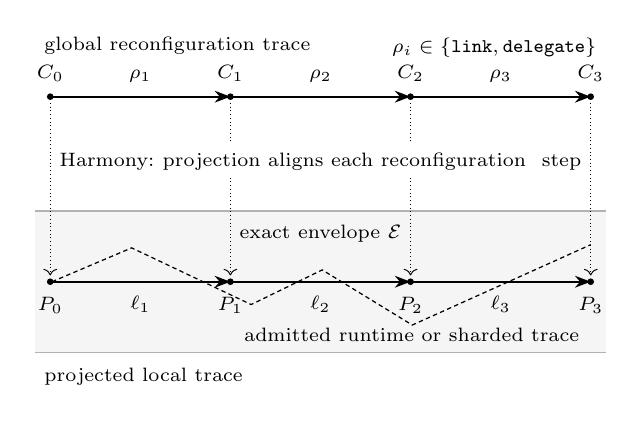
\begin{tikzpicture}[x=1.1mm,y=1mm,figfont]
				% Exact envelope corridor around local trace
					\fill[gray!8] (-33,-11.5) rectangle (33,6.5);
					\draw[gray!60, line width=0.5pt] (-33,6.5) -- (33,6.5);
					\draw[gray!60, line width=0.5pt] (-33,-11.5) -- (33,-11.5);
					\node[font=\scriptsize, align=center] at (0,3.6) {exact envelope $\mathcal{E}$};

			% Top: global reconfiguration trace
					\node[font=\scriptsize, anchor=west] at (-33,27.5) {global reconfiguration trace};
				\fill (-31.2,21.0) circle (1.2pt) node[above=2.0pt] {$C_0$};
				\fill (-10.4,21.0) circle (1.2pt) node[above=2.0pt] {$C_1$};
				\fill (10.4,21.0) circle (1.2pt) node[above=2.0pt] {$C_2$};
				\fill (31.2,21.0) circle (1.2pt) node[above=2.0pt] {$C_3$};
				\draw[figarrowstrong] (-31.2,21.0) -- node[above=1.5pt, font=\scriptsize] {$\rho_1$} (-10.4,21.0);
				\draw[figarrowstrong] (-10.4,21.0) -- node[above=1.5pt, font=\scriptsize] {$\rho_2$} (10.4,21.0);
				\draw[figarrowstrong] (10.4,21.0) -- node[above=1.5pt, font=\scriptsize] {$\rho_3$} (31.2,21.0);
					\node[font=\scriptsize, anchor=east] at (33,27.2)
					{$\rho_i\in\{\texttt{link}, \texttt{delegate}\}$};

			% Bottom: projected local trace
				\node[font=\scriptsize, anchor=west] at (-33,-14.6) {projected local trace};
				\fill (-31.2,-2.5) circle (1.2pt) node[below=2.0pt] {$P_0$};
				\fill (-10.4,-2.5) circle (1.2pt) node[below=2.0pt] {$P_1$};
				\fill (10.4,-2.5) circle (1.2pt) node[below=2.0pt] {$P_2$};
				\fill (31.2,-2.5) circle (1.2pt) node[below=2.0pt] {$P_3$};
				\draw[figarrowstrong] (-31.2,-2.5) -- node[below=1.5pt, font=\scriptsize] {$\ell_1$} (-10.4,-2.5);
				\draw[figarrowstrong] (-10.4,-2.5) -- node[below=1.5pt, font=\scriptsize] {$\ell_2$} (10.4,-2.5);
				\draw[figarrowstrong] (10.4,-2.5) -- node[below=1.5pt, font=\scriptsize] {$\ell_3$} (31.2,-2.5);

			% Projection alignments (Harmony correspondences)
				\draw[densely dotted, ->, line width=0.35pt] (-31.2,20.2) -- (-31.2,-1.7);
				\draw[densely dotted, ->, line width=0.35pt] (-10.4,20.2) -- (-10.4,-1.7);
				\draw[densely dotted, ->, line width=0.35pt] (10.4,20.2) -- (10.4,-1.7);
				\draw[densely dotted, ->, line width=0.35pt] (31.2,20.2) -- (31.2,-1.7);
				\node[font=\scriptsize, align=center] at (0,12.8)
				{Harmony:\colorbox{white}{projection aligns each reconfiguration} step};

				% In-band admissible runtime trace (piecewise-linear, crossing local transitions)
				\draw[dash pattern=on 1.6pt off 1.2pt, line width=0.45pt]
				(-31,-2.5) -- (-21.8,1.8) -- (-8,-5.4) -- (0.2,-1.0) --
				(10.6,-8) -- (31.2,2.2);
				\node[font=\scriptsize, align=right, anchor=east] at (31,-9.2)
				{admitted runtime or sharded trace};
		\end{tikzpicture}
		\caption{Dual-track trace view: reconfiguration steps and projected local steps align under Harmony, while admitted runtime traces remain inside the exact envelope.}
		\label{fig:p3-layered-stack}
	\end{figure}

The determinism-envelope layer follows a standard refinement-bound idea. One defines an admissible
behavior relation that captures implementation freedom while preserving safety-visible observations.
What is new here is an exact characterization for asynchronous MPST reconfiguration with soundness,
realizability, and maximality proved in one theorem stack and connected directly to runtime admission
and adherence evidence (Abadi and Lamport, 1991; Alpern and Schneider, 1985).

Equivalently, the envelope is a coarse-grained observational equivalence. It is the maximal admissible
blur between executions that still preserves certified safety-visible meaning, in the spirit of
noninterference and hyperproperty viewpoints (Goguen and Meseguer, 1982; Clarkson and Schneider, 2010).

Sharding correspondence follows a standard simulation view for distributed execution. A split execution
should preserve the same safety-visible meaning as a reference execution under explicit compatibility
assumptions (Lamport, 1978; Chandy and Lamport, 1985; Lynch, 1996). What is new here is an explicit
envelope contract for local and cross-machine sharding profiles that makes the admissible difference
class theorem-checkable and capability-gated at the VM bridge.

The envelope layer also admits a rate-distortion style reading. The reference semantics is the source,
VM and sharded executions are channels, and admission profiles are distortion constraints on safety-visible
observations (Shannon, 1948, and Cover and Thomas, 2006). Maximality then states that no strictly larger
distortion class preserves the same certified safety guarantees.

This paper closes the series architecture. \emph{Coherence for Asynchronous Buffered MPST} supplies
the invariant kernel. \emph{Computable Dynamics for Asynchronous MPST} supplies bounds and decision
procedures. This paper supplies reconfiguration commutation and envelope-level runtime adherence.

Terminology note. In classical MPST, coherence primarily names global-type coherence and projectability
conditions, with later refinements of projection criteria (Honda et al., 2008; Honda et al., 2016;
Castagna et al., 2012; Majumdar et al., 2021). Logical lines also formulate
coherence as n-ary duality or proof compatibility (Carbone et al., 2015; Carbone et al., 2016; Carbone
et al., 2017), and data-certification extensions remain in the same global-projection discipline
(Toninho and Yoshida, 2017). In this paper, as in \emph{Coherence for Asynchronous Buffered MPST}, $\Coherent$ denotes
the inherited operational invariant on local environments and buffered traces, and the contribution is a
reconfiguration and envelope theorem stack over that refined operational form.

Scope is confined to asynchronous buffered semantics with explicit reconfiguration conditions,
crash-stop fault assumptions where fault claims are stated, and declared envelope-admission profiles.

Our contributions are as follows:
\begin{enumerate}
	\item A reconfiguration commutation theorem that covers both static composition and dynamic delegation.
	\item An exact characterization of Coherence by active-edge erasure realizability and a relative-minimality theorem over admissible invariants.
	\item A determinism-envelope theory with soundness, realizability, maximality, and exchange and spatial normalization consequences.
	\item An abstract-to-VM adequacy bridge that ties profile claims to theorem-pack capability evidence.
	\item A Byzantine envelope extension with exact characterization, converse counterexample families, and capability-gated VM adherence.
\end{enumerate}

\begin{table}[H]
	\centering
	\small
			\begin{tabularx}{\columnwidth}{@{}L{0.36\columnwidth}L{0.59\columnwidth}@{}}
			\toprule
			\thead{Symbol}   & \thead{Meaning}                      \\
			\midrule
			$\Hbyz$          & Byzantine characterization bundle    \\
			$\Obssafe$       & Byzantine safety-visible observation \\
			$\Eqsafe$        & Byzantine safety-visible equality    \\
			$\Ebyz$          & Byzantine determinism-envelope       \\
			\Coherent        & global active-edge coherence predicate \\
			\Harmony         & reconfiguration commutation invariant \\
			$\Admissible(I)$ & candidate invariant admissibility    \\
			$W$              & weighted state function              \\
			$\mathcal{E}$    & determinism envelope relation        \\
				\EnvelopeRel     & envelope relation between VM and reference states \\
				\EnvelopeExact   & exactness of envelope characterization \\
				\EnvelopeOK      & envelope-admission predicate            \\
				\ConfigEquiv{}   & erasure-stability equivalence        \\
				\Obs             & observation map on executions/states \\
				\ByzChar         & Byzantine characterization formula    \\
				\ByzSafe         & Byzantine safety predicate            \\
				\HasProfileCapabilities & theorem-pack capability-evidence predicate \\
				\VMAdheres       & VM adherence predicate under admitted profile \\
				$\rho$           & reconfiguration step label (link/delegate/transition) \\
			\bottomrule
		\end{tabularx}
	\caption{Notation used in this paper.}
	\label{tab:p3-notation}
\end{table}

% ============================================================================
\section{Setup, Definitions, and Side Conditions}
\label{sec:setup}
% ============================================================================

\subsection{Base Recap}

Assume the base model from \emph{Coherence for Asynchronous Buffered MPST} and \emph{Computable Dynamics for Asynchronous MPST}:
\begin{itemize}
	\item asynchronous buffered steps,
	\item active-edge Coherence,
	\item fair scheduling assumptions stated per theorem,
	\item \texttt{DeliveryModel} parametricity,
	\item crash-stop setting for fault claims.
\end{itemize}

\begin{table}[H]
	\centering
	\small
	\begin{tabularx}{\columnwidth}{@{}L{0.55\columnwidth}L{0.4\columnwidth}@{}}
		\toprule
		\thead{Assumption}                          & \thead{Status}         \\
		\midrule
		async buffered semantics                    & required               \\
		active-edge Coherence                       & required               \\
		reconfig.\ conditions \texttt{DelegationWF} & required               \\
		fair scheduling profile                     & req.\ where stated     \\
		crash-stop fault model                      & req.\ for fault claims \\
		\bottomrule
	\end{tabularx}
	\caption{Model assumptions for exact claims in this paper.}
	\label{tab:p3-model-assumptions}
\end{table}

\begin{assumptions}[Core Model]
	\label{assump:p3-core}
	Core claims in this paper assume asynchronous buffered semantics, active-edge Coherence,
	reconfiguration side conditions through \texttt{DelegationWF}, and the stated fairness profile.
	Crash-stop premises apply where fault-side claims are stated.
\end{assumptions}

\subsection{Reconfiguration Operators}

The paper distinguishes:
\begin{itemize}
	\item static composition (\texttt{link}) in deployment-level composition,
	\item dynamic delegation (endpoint/capability transfer during execution).
\end{itemize}

Representative mechanized anchors are in the deployment-composition layer, the delegation-preservation
layer, and the higher-order graph-delta layer. Appendix~\ref{app:mechanization} provides the file-level mapping.

\subsection{Dynamic Participant Sets}

Participant sets are not fixed:
\begin{itemize}
	\item joining through delegation,
	\item leaving through crash-stop or transfer-and-exit,
	\item topology change through composition.
\end{itemize}

The objective is to preserve Coherence/Harmony across these mutations.

\subsection{Core Definitions}

Write $\envG(C)$ and $\envD(C)$ for the global and delayed-trace environments extracted from
configuration $C$, and $\Obs$ for the safety-visible observation map.

\begin{definition}[Lifted Coherence]
	\begin{equation}
		\Coherent(C) := \Coherent(\envG(C), \envD(C)).
	\end{equation}
\end{definition}

\begin{definition}[Harmony]
	For reconfiguration operator $\rho$,
	\begin{equation}
		\begin{aligned}[t]
			\Harmony(C,\rho)
			 & :\iff \ProjStep{C}{\rho} \\
			 & =
			\LocStep{C}{\rho}.
		\end{aligned}
	\end{equation}
\end{definition}

Here $\ProjStep{C}{\rho}$ abbreviates
$\mathsf{project}(\mathsf{step}_{\mathsf{reconfig}}(C,\rho))$,
and $\LocStep{C}{\rho}$ abbreviates
$\mathsf{localStep}_{\mathsf{reconfig}}(\mathsf{project}(C),\rho)$.

Figure~\ref{fig:p3-commuting-square} gives the explicit commuting-square instance for Harmony.
\begin{figure}[H]
	\centering
		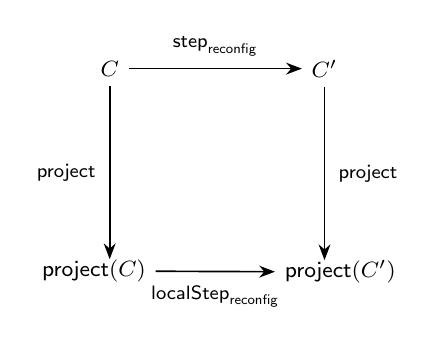
\begin{tikzpicture}[figfont, node distance=22mm]
			% Corner nodes
			\node[font=\footnotesize\sffamily] (TL) {$C$};
			\node[right=of TL, font=\footnotesize\sffamily] (TR) {$C'$};
			\coordinate[below=of TL] (BL);
			\coordinate[below=of TR] (BR);
			\node[font=\footnotesize\sffamily, xshift=-2mm, yshift=-1.5mm] (BLlbl) at (BL) {$\mathsf{project}(C)$};
			\node[font=\footnotesize\sffamily, xshift=2mm, yshift=-1.5mm] (BRlbl) at (BR) {$\mathsf{project}(C')$};

		% Horizontal arrows
			\draw[figarrowstrong] (TL) -- node[above=1.0pt, font=\scriptsize] {$\mathsf{step}_{\mathsf{reconfig}}$} (TR);
			\draw[figarrowstrong] (BLlbl) -- node[below=1.5pt, font=\scriptsize] {$\mathsf{localStep}_{\mathsf{reconfig}}$} (BRlbl);

		% Vertical arrows
			\draw[figarrowstrong] (TL) -- node[left=1.5pt, font=\scriptsize] {$\mathsf{project}$} (BL);
			\draw[figarrowstrong] (TR) -- node[right=1.5pt, font=\scriptsize] {$\mathsf{project}$} (BR);
		\end{tikzpicture}

	\vspace{4pt}
	{\footnotesize $\rho\in\{\mathsf{link},\mathsf{delegate}\}$}
	\caption{Commuting-square formulation of Harmony.}
	\label{fig:p3-commuting-square}
\end{figure}

\begin{definition}[Joint Realizability on Active Edges]
	$\mathsf{JointRealizable}_{\mathsf{active}}(\mathsf{project}(C))$ holds when projected
	local views admit witnesses for all active edges.
\end{definition}

\begin{definition}[Reconfiguration Well-Formedness]
	Write $\mathsf{WF}_\rho(C)$ for the side-condition predicate used by reconfiguration theorems:
	\texttt{LinkWF(C,$\rho$)} for static linking, \texttt{DelegationWF(C,$\rho$)} for delegation,
	and \texttt{TransitionWF(C,$\rho$)} for transition choreographies.
\end{definition}

\begin{definition}[Delegation Safety Predicates]
	$\mathsf{SafeDelegation}(C,op)$ is the global delegation-safety judgment, and
	$\mathsf{SafeDelegationFootprint}(C,op)$ is its footprint-local form over edges touched by $op$.
\end{definition}

\begin{definition}[$\Admissible(I)$]
	Locality plus erasure stability (\ConfigEquiv) plus frame stability plus delegation adequacy.
\end{definition}

\begin{definition}[Envelope Predicates]
	$\EnvelopeRel(S_{\mathrm{vm}}, S_{\mathrm{ref}})$ is the envelope relation between VM and
	reference states. $\EnvelopeExact(C)$ is exactness of the declared envelope (soundness and
	realizability and maximality) at configuration $C$. $\EnvelopeOK(C)$ means $C$ satisfies
	the envelope-admission obligations used in Theorems~\ref{thm:envelope}--\ref{thm:normalization}.
\end{definition}

\begin{definition}[Capability/Adherence Predicates]
	$\HasProfileCapabilities(P,\Pi)$ means profile $(P,\Pi)$ is backed by required theorem-pack
	capability evidence. $\VMAdheres(P,\Pi)$ means executions admitted under $(P,\Pi)$ satisfy
	the corresponding adherence obligations.
\end{definition}

\begin{definition}[Normalization Relations]
	$\ExchangeEq(C_1,C_2)$ is exchange equivalence modulo admissible reordering.
$C \sqsubseteq_{\mathsf{sp}} C'$ is the spatial-subtyping preorder used in Theorem~\ref{thm:normalization}.
\end{definition}

Equation~\ref{eq:p3-delegation-footprint} states the delegation-footprint update discipline.
\begin{equation}
	\label{eq:p3-delegation-footprint}
	\begin{aligned}[t]
		\forall e\in \mathsf{Footprint}(op),\quad
		D'(e) & =\mathsf{rewrite}(D(e),op); \\
		\forall e\notin \mathsf{Footprint}(op),\quad
		D'(e) & =D(e)\land G'(e)=G(e).
	\end{aligned}
\end{equation}

% ============================================================================
\section{Worked Example}
\label{sec:example}
% ============================================================================

We use one running example that carries the full structural theorem stack (\ABHStack).

\noindent\begingroup\raggedright
\textbf{Running example.} Baseline choreography:
\par\endgroup

\noindent\begin{minipage}{\columnwidth}
	\begin{lstlisting}
C -> P : Request(n)
P -> C : Grant(k)
C -> M : Report(k)
M -> P : Confirm
P -> C : Token(t)
\end{lstlisting}
\end{minipage}

Extended system adds: \texttt{link} federation (\texttt{P1}, \texttt{P2}),
delegation $C \to C'$, and optimistic-to-coordinated transition choreography.

Fix configurations and reconfiguration operators:
\begin{equation}
	C_0 \xrightarrow{\rho_{\mathsf{link}}} C_1 \xrightarrow{\rho_{\mathsf{del}}}
	C_2 \xrightarrow{\rho_{\mathsf{tr}}} C_3.
\end{equation}
Assume well-formedness judgments $\Gamma \vdash C_i\ \wf$ for $i=0,1,2,3$.

\begin{itemize}
	\item $C_0$: coherent single-pool state before federation.
	\item $C_1$: linked/federated state.
	\item $C_2$: post-delegation state where token capability is held by $C'$.
	\item $C_3$: coordinated-mode state after transition choreography.
\end{itemize}

The running obligations are used through these derived rule instances.
Write $\mathsf{TrPrem}(C)$ for the transition-profile premise package at $C$, and
$\mathsf{BDesc}(C,C')$ for a budget-certified descent witness from $C$ to $C'$.

	{\small
		\begin{equation}
			\begin{aligned}
				\mathsf{SD}(C,\rho)        & := \mathsf{SafeDelegation}(C,\rho);                      \\
			\mathsf{SDF}(C,\rho)       & := \mathsf{SafeDelegationFootprint}(C,\rho);             \\
			\mathsf{EnvRel}^{\star}(C) & := \EnvelopeRel(S_{\mathsf{vm}}(C),S_{\mathsf{ref}}(C)); \\
			\mathsf{ObsEq}^{\star}(C)  & := \Obs(S_{\mathsf{vm}}(C))=\Obs(S_{\mathsf{ref}}(C)).
		\end{aligned}
	\end{equation}
}
\eqnote{Example derivation: link harmony}
	{\small
		\begin{equation}
			\dfrac{
				\Gamma \vdash C_0\ \wf;\ \mathsf{WF}_{\rho_{\mathsf{link}}}(C_0)
		}{
			\ProjStep{C_0}{\rho_{\mathsf{link}}}
			=
			\LocStep{C_0}{\rho_{\mathsf{link}}}
		}
	\end{equation}
}
\eqnote{Example derivation: delegation safety}
	{\small
		\begin{equation}
			\dfrac{
				\Coherent(C_1);\ \mathsf{DelegationWF}(C_1,\rho_{\mathsf{del}})
		}{
			\mathsf{SD}(C_1,\rho_{\mathsf{del}});\ \mathsf{SDF}(C_1,\rho_{\mathsf{del}})
		}
	\end{equation}
}
\eqnote{Example derivation: conservation}
	{\small
		\begin{equation}
			\dfrac{
				\mathsf{WF}_{\rho_{\mathsf{link}}}(C_0);\ \Coherent(C_0)
		}{
			W(C_1)=W(C_0)
		}
	\end{equation}
}
\eqnote{Example derivation: transition}
{\small
			\begin{equation}
				\dfrac{
					\mathsf{WF}_{\rho_{\mathsf{tr}}}(C_2);\ \Coherent(C_2);\ \mathsf{TrPrem}(C_2)
				}{
					C_2 \to^\ast C_3;\ \mathsf{BDesc}(C_2,C_3)
				}
			\end{equation}
	}
\eqnote{Example derivation: adequacy and adherence}
		{\small
			\begin{equation}
				\dfrac{
					\mathsf{EnvRel}^{\star}(C_3);\ \HasProfileCapabilities(P,\Pi)
			}{
				\mathsf{ObsEq}^{\star}(C_3);\ \VMAdheres(P,\Pi)
			}
		\end{equation}
}

Table~\ref{tab:p3-typed-guards} gives the typed guard clauses used to discharge $\mathsf{WF}_{\rho_{\mathsf{tr}}}$
for the optimistic-to-coordinated step.

\begin{table}[H]
	\centering
	\footnotesize
	\begin{tabularx}{\columnwidth}{@{}L{0.3\columnwidth}L{0.33\columnwidth}L{0.27\columnwidth}@{}}
		\toprule
		\thead{Guard}                                 & \thead{Source}          & \thead{Consequence} \\
		\midrule
			\texttt{conflict\_detected}                   & app-level trigger       & transition enabled  \\
		\texttt{reachable}\allowbreak\texttt{(Coord)} & crash-tolerance decider & path not cut        \\
		$W \leq \text{budget}$                        & quant.\ bound           & completes in budget \\
		$|F| \leq f$                                  & fault-budget decl.      & bounded tolerance   \\
		\bottomrule
	\end{tabularx}
	\caption{Typed guard clauses for transition well-formedness.}
	\label{tab:p3-typed-guards}
\end{table}

Concrete reading: $C_0$ pre-federation, $C_1$ linked, $C_2$ post-delegation handoff, $C_3$
coordinated mode with preserved envelope obligations.

% ============================================================================
\section{Theorem B: Reconfiguration Harmony (Static + Dynamic)}
\label{sec:theorem-b}
% ============================================================================

\begin{assumptions}[Reconfiguration]
	\label{assump:p3-reconfiguration}
	The reconfiguration theorems assume typed global and local states, reconfiguration
	witnesses satisfying \texttt{DelegationWF}, enabled post-reconfiguration steps, and
	compatibility side conditions for unaffected edges.
\end{assumptions}

\begin{theorem}[Reconfiguration Harmony]
	\label{thm:harmony}
	For all configurations $C$ and reconfiguration operators $\rho \in \{\mathsf{link},
		\mathsf{delegate}\}$, if Assumption Block~\ref{assump:p3-reconfiguration} holds for $(C,\rho)$, then
	\begin{equation}
		\ProjStep{C}{\rho}
		=
		\LocStep{C}{\rho}.
	\end{equation}
	Equivalently, the reconfiguration square commutes at the projection boundary.
\end{theorem}

The proof has two components.
\begin{enumerate}
	\item Static Harmony via \texttt{link}. Composition-level commutation and coherence
	      preservation are established in deployment theorems, for example
	      \nolinkurl{link_harmony_through_link} and \nolinkurl{link_preserves_coherent}.
	\item Dynamic Harmony via delegation. Delegation preservation and renaming and
	      footprint lemmas establish commutation for topology-changing transfers.
\end{enumerate}

At the effect-observation boundary, the coinductive bridge supplies the composition-facing
congruence and quotient lift used by this section: \nolinkurl{effectBisim_congr_link} and
\nolinkurl{configEquiv_iff_effectBisim_silent}.

Side-condition necessity is explicit. Dropped-condition counterexample interfaces are part
of the reconfiguration bridge layer.

\begin{proof}[Proof sketch]
	The theorem is proved by decomposition over reconfiguration operators.

	\begin{enumerate}
		\item \texttt{link} case:
		      \begin{itemize}
			      \item construct composed deployment object under link well-formedness,
			      \item apply composition-preservation and harmony lemmas (\nolinkurl{link_preserves_coherent},\allowbreak\ \nolinkurl{link_harmony_through_link}),
			      \item transport equality to projected local-step view.
		      \end{itemize}
		\item \texttt{delegate} case:
		      \begin{itemize}
			      \item apply delegation-preservation and footprint-local update lemmas,
			      \item show only footprint edges are rewritten; unrelated edges are frame-preserved,
			      \item commute projection with the delegated local transition.
		      \end{itemize}
		\item Quotient/effect boundary:
		      \begin{itemize}
			      \item use effect-bisim congruence under link and quotient bridge (\nolinkurl{effectBisim_congr_link},\allowbreak\ \nolinkurl{configEquiv_iff_effectBisim_silent}) to align protocol and observational views.
		      \end{itemize}
	\end{enumerate}

	Hence reconfigured global evolution and projected local evolution commute under Assumption Block~\ref{assump:p3-reconfiguration}.
\end{proof}

Equation~\ref{eq:p3-commutation-instances} separates static-link and dynamic-delegation commutation instances.
\eqnote{Commutation instances: link and delegate}
\begin{equation}
	\label{eq:p3-commutation-instances}
	\begin{aligned}[t]
		\ProjLink{C} & = \LocLink{C};     \\
		\ProjDelegate{C} & = \LocDelegate{C}.
	\end{aligned}
\end{equation}

% ============================================================================
\section{Theorem A: Erasure Characterization of Coherence}
\label{sec:theorem-a}
% ============================================================================

\begin{theorem}[Erasure Characterization of Coherence]
	\label{thm:erasure}
	For all configurations $C$ with global and delayed environments $(G,D)$,
	\begin{equation}
		\begin{aligned}[t]
			\Coherent(G,D)
			\\
			\iff\ \JointActive{\mathsf{project}(C)}.
		\end{aligned}
	\end{equation}
	That is, Coherence holds exactly when projected local views admit a compatible active-edge witness assignment.
\end{theorem}

Mechanized anchors include \nolinkurl{coherent_erasure_stable} and its companion characterization lemmas.

This theorem gives the formal content of the quotient-first claim: erasure is not a heuristic post-processing step but the semantic object preserved by the theorem stack.

\begin{proof}[Proof sketch]
	The two directions are proved separately.

	\begin{enumerate}
		\item $\Coherent \to \mathsf{JointRealizable}_{\mathsf{active}}$:
		      \begin{itemize}
			      \item from edge-local compatibility ($\mathsf{EdgeCoherent}$) build per-edge witnesses for projected local obligations,
			      \item combine witnesses over active edges to obtain joint realizability.
		      \end{itemize}
		\item $\mathsf{JointRealizable}_{\mathsf{active}} \to \Coherent$:
		      \begin{itemize}
			      \item invert witness assignment into edge-local consume compatibility,
			      \item reassemble edge obligations into global $\Coherent$.
		      \end{itemize}
		\item Erasure stability:
		      \begin{itemize}
			      \item use \nolinkurl{coherent_erasure_stable} to show equivalence is preserved across configuration erasure classes.
		      \end{itemize}
	\end{enumerate}

	Therefore Coherence is exactly characterized by active-edge realizability of projected views.
\end{proof}

% ============================================================================
\section{Theorem C: Safe Delegation Corollary}
\label{sec:theorem-c}
% ============================================================================

\begin{theorem}[Safe Delegation Sufficiency]
	\label{thm:delegation}
	For all configurations $C$ and delegation operations $op$,
	\begin{equation}
		\begin{aligned}[t]
			\Coherent(C) \land \mathsf{DelegationWF}(C,op)
			\\
			\implies\ \mathsf{SafeDelegation}(C,op).
		\end{aligned}
	\end{equation}
\end{theorem}

\begin{corollary}[Footprint Exactness Packaging]
	\label{cor:footprint}
	For all $C,op$ satisfying the stated step and well-formedness side conditions,
	\begin{equation}
		\begin{aligned}[t]
			\mathsf{SafeDelegation}(C,op)
			\\
			\iff\ \mathsf{SafeDelegationFootprint}(C,op).
		\end{aligned}
	\end{equation}
	The converse direction is accompanied by strictness witnesses for dropped side conditions.
\end{corollary}

Mechanized anchors:
\begin{itemize}
	\item \nolinkurl{safeDelegation_local_necessity}
	\item \nolinkurl{safeDelegation_to_footprint}
	\item \nolinkurl{footprint_to_safeDelegation}
	\item \nolinkurl{safeDelegation_iff_footprint}
\end{itemize}

These lemmas are grouped in the erasure-characterization layer.

\begin{proof}[Proof sketch]
	Sufficiency follows by composing:
	\begin{enumerate}
		\item Coherence on active edges,
		\item delegation well-formedness side conditions (\texttt{DelegationWF}),
		\item delegation-preservation lemmas that update only the delegation footprint.
	\end{enumerate}
	Together these imply safe delegation without introducing additional global invariants.
\end{proof}

\begin{proof}[Proof sketch]
	For the forward direction, instantiate Theorem~\ref{thm:delegation} and project its obligations to the declared delegation footprint. For the reverse direction, apply \nolinkurl{footprint_to_safeDelegation} to reconstruct global safety from footprint obligations, then use strictness witnesses to show necessity of the side conditions. Combining both implications yields the stated equivalence.
\end{proof}

% ============================================================================
\section{Theorem D: Relative Minimality}
\label{sec:theorem-d}
% ============================================================================

\begin{theorem}[Relative Minimality]
	\label{thm:minimality}
	For all invariants $I$,
	\begin{equation}
		\begin{aligned}[t]
			\Admissible(I)
			 & \implies \forall C,\ I(C) \\
			 & \implies \Coherent(C).
		\end{aligned}
	\end{equation}
	Hence Coherence is the weakest admissible invariant that guarantees delegation safety under the stated model side conditions.
\end{theorem}

Mechanized anchors:
\begin{itemize}
	\item \nolinkurl{relative_minimality}
	\item supporting witness and counterexample lemmas in the minimality layer
\end{itemize}

This theorem prevents ``stronger-than-needed'' invariant inflation and pins down the architectural core.

\begin{proof}[Proof sketch]
	Assume any invariant $I$ satisfying $\Admissible(I)$.

	\begin{enumerate}
		\item Use admissibility clauses (locality, erasure stability, frame stability, delegation adequacy) to transport $I$ along the same edge-local transformations used by Coherence.
		\item Apply delegation-safety adequacy to derive local safety obligations on all active edges.
		\item Convert these obligations into Coherence via erasure-characterization lemmas.
	\end{enumerate}

	Hence every admissible safety-guaranteeing invariant implies Coherence, making Coherence relatively minimal.
\end{proof}

Equation~\ref{eq:p3-admissible-order} summarizes the admissible-invariant order behind Theorem~\ref{thm:minimality}.
\begin{equation}
	\label{eq:p3-admissible-order}
	\begin{array}{c}
		\Admissible(I)
		\\
		\Downarrow
		\\
		\forall C,\ I(C)\Rightarrow \Coherent(C)
		\\
		\Downarrow
		\\
		\text{delegation safety consequences}.
	\end{array}
\end{equation}

% ============================================================================
\section{Theorem E: Composed-System Conservation}
\label{sec:theorem-e}
% ============================================================================

\begin{theorem}[Composed-System Conservation]
	\label{thm:conservation}
	For all configurations $C$ and reconfiguration operators $\rho$, if $\mathsf{WF}_\rho(C)$ and $\Coherent(C)$ hold, then
	\begin{equation}
		\Coherent(\mathsf{step}_{\mathsf{reconfig}}(C,\rho)).
	\end{equation}
	For all configurations $C$ and pure reconfiguration operators $\rho$,
	\begin{equation}
		\begin{aligned}[t]
			\mathsf{WF}_\rho(C) \land \Coherent(C)
			\\
			\implies\ W(\mathsf{step}_{\mathsf{reconfig}}(C,\rho)) = W(C).
		\end{aligned}
	\end{equation}
	For transition choreographies $\rho_{\mathrm{tr}}$ with stated budget and scheduler premises, descent and budget certificates are preserved with conservative profile-dependent bounds.
\end{theorem}

The theorem separates conservation and dissipation roles. Pure reconfiguration preserves the weighted quantity exactly. Transition choreographies consume certified progress budget and are therefore dissipative with explicit bounds. This split keeps structural rewiring distinct from progress-consuming work.

Under composition and delegation:
\begin{enumerate}
	\item Coherence and Harmony are preserved.
	\item Quantitative lift from \emph{Computable Dynamics for Asynchronous MPST} holds:
	      \begin{itemize}
		      \item pure reconfiguration conserves the weighted measure,
		      \item transition choreographies are governed by descent and budget certificates.
	      \end{itemize}
\end{enumerate}

Mechanized anchors:
\begin{itemize}
	\item \nolinkurl{flagship_composed_system_conservation}
	\item \nolinkurl{lyapunov_conserved_under_balanced_delegation}
\end{itemize}

This theorem combines composition, delegation, and quantitative invariants in one package.

\begin{proof}[Proof sketch]
	Split reconfiguration into conservative and budgeted classes.

	\begin{enumerate}
		\item Pure reconfiguration (\texttt{link}/delegation):
		      \begin{itemize}
				      \item preserve Coherence/Harmony by Theorem~\ref{thm:harmony}-side machinery,
			      \item show weighted measure $W$ is invariant under balanced delegation/rewiring (\nolinkurl{lyapunov_conserved_under_balanced_delegation}).
		      \end{itemize}
		\item Transition choreographies:
		      \begin{itemize}
			      \item apply inherited quantitative descent/budget certificates from the dynamics layer,
			      \item conclude bounded dissipation under declared scheduler premises.
		      \end{itemize}
		\item Compose both cases to obtain theorem statement and conservative profile-dependent quantitative side.
	\end{enumerate}
\end{proof}

\begin{corollary}[Compositional Exactness Under Non-Interference]
	\label{cor:compositional}
	For all compositions $C_1 \otimes C_2$, if non-interference premises hold across the composition boundary, then envelope exactness is preserved by composition:
	\begin{equation}
		\begin{aligned}
			\EnvelopeExact(C_1) \land \EnvelopeExact(C_2)
			 & \implies \\
			\EnvelopeExact(C_1 \otimes C_2).
		\end{aligned}
	\end{equation}
	Strictness witnesses are provided for dropped non-interference premises.
\end{corollary}

\begin{proof}[Proof sketch]
	Non-interference gives a factorization of composed traces into component traces with no cross-boundary interference steps. Apply envelope exactness to each component and recompose to obtain exactness of the composition. For strictness, use the dropped-assumption witness family to exhibit an interfering trace that violates factorization and therefore exactness.
\end{proof}

Equation~\ref{eq:p3-quantitative-split} summarizes the quantitative split.
	\begin{equation}
		\label{eq:p3-quantitative-split}
		\begin{aligned}[t]
			\text{pure reconfiguration}
			 & \Rightarrow W(\mathsf{step}_{\mathsf{reconfig}}(C,\rho)) = W(C); \\
			\text{transition choreography}
			 & \Rightarrow \text{descent/budget certificate}.
		\end{aligned}
	\end{equation}
Pure reconfiguration preserves $W$, while transition choreographies satisfy the inherited descent/budget inequality under stated profile assumptions.

% ============================================================================
\section{Theorem F: Exact Characterization of Determinism Envelope}
\label{sec:theorem-f}
% ============================================================================

\begin{assumptions}[Envelope]
	\label{assump:p3-envelope}
	Envelope theorems assume the declared admissibility profile with trace well-formedness, certified-step obligations, and the realizability witness schema used by the admission checker.
\end{assumptions}

\begin{theorem}[Exact Determinism Envelope]
	\label{thm:envelope}
	Under Assumption Block~\ref{assump:p3-envelope}, there exists an envelope relation $\mathcal{E}$ such that:
	\begin{enumerate}
		\item Soundness: $\forall t,\ \mathsf{Certified}(t) \implies t \in \mathcal{E}$.
		\item Realizability: $\forall t \in \mathcal{E},\ \exists e,\ \mathsf{Trace}(e) = t$.
		\item Maximality: $\forall \mathcal{E}'$, if $\mathcal{E}' \supsetneq \mathcal{E}$, then $\exists t \in \mathcal{E}' \setminus \mathcal{E}$ that violates admissibility constraints.
	\end{enumerate}
\end{theorem}

The envelope claim is exact under the stated model and assumption bundle:
\begin{enumerate}
	\item soundness: certified executions lie within the envelope.
	\item realizability and completeness: admitted envelope behaviors are witnessed.
	\item maximality: strict supersets are rejected by witness counterexamples.
\end{enumerate}

Conceptually, this is dual to Theorem~\ref{thm:minimality}:
\begin{itemize}
	\item D: weakest admissible invariant core,
	\item F: maximal admissible behavior envelope.
\end{itemize}

Mechanized envelope bridge layers include core foundations, admission logic, and reconfiguration bridge components.

\begin{proof}[Proof sketch]
	Exactness is obtained by packaging three envelope properties.

	\begin{enumerate}
		\item Soundness:
		      \begin{itemize}
			      \item derive $\mathsf{Certified} \to \mathsf{Envelope}$ from local/sharded envelope soundness definitions and profile extraction.
		      \end{itemize}
		\item Realizability/completeness:
		      \begin{itemize}
			      \item use realizability witness schemas to construct executions for admitted envelope behaviors.
		      \end{itemize}
		\item Maximality:
		      \begin{itemize}
			      \item show any strict envelope extension violates admissibility via explicit witness obligations.
		      \end{itemize}
	\end{enumerate}

	Core formal structures come from envelope foundations (\texttt{LocalExactEnvelopeCharacterization}, \texttt{ShardedExactEnvelopeCharacterization}) and profile-level extraction theorems (\nolinkurl{consensusEnvelope_exact_of_profile},\allowbreak\ \nolinkurl{failureEnvelope_maximality_of_profile}).
\end{proof}

\begin{corollary}[Finite-Erasure Transportability Boundary]
	\label{cor:transportability}
	Under stated model assumptions,
	\begin{equation}
		\begin{aligned}[t]
			\forall t,\ \mathsf{FiniteErasureTransportable}(t)
			\\
			\iff\ \mathsf{RationalFiniteState}(t).
		\end{aligned}
	\end{equation}
\end{corollary}

\begin{corollary}[Strict Boundary Witness]
	\label{cor:boundary}
	There exists $t$ such that
	\begin{equation}
		\begin{aligned}[t]
			\neg \mathsf{RationalFiniteState}(t)
			\\
			\land\ \neg \mathsf{FiniteErasureTransportable}(t).
		\end{aligned}
	\end{equation}
\end{corollary}

\begin{corollary}[Inductive-Embedding Exactness]
	\label{cor:embedding}
	For all inductive states $x$, exact envelope characterization is preserved under \texttt{toCoind}:
	\begin{equation}
		\begin{aligned}[t]
			\EnvelopeExact_{\mathrm{ind}}(x)
			\\
			\iff\ \EnvelopeExact_{\mathrm{coind}}(\mathsf{toCoind}(x)).
		\end{aligned}
	\end{equation}
\end{corollary}

Appendices~\ref{app:regimes} and~\ref{app:consequences} provide the detailed witness constructions and transport lemmas for these boundary corollaries.

% ============================================================================
\section{Theorem G: Exchange-Normalized Determinism and Spatial Monotonicity}
\label{sec:theorem-g}
% ============================================================================

\begin{theorem}[Exchange-Normalized Determinism and Spatial Monotonicity]
	\label{thm:normalization}
	For all configurations under envelope premises, the following properties hold:
	\begin{enumerate}
		\item Exchange normalization:
		      \begin{equation}
			      \begin{aligned}[t]
				      \ExchangeEq(C_1,C_2)
				      \\
				      \implies\ \Obs(C_1) = \Obs(C_2).
			      \end{aligned}
		      \end{equation}
		\item Spatial monotonicity:
		      \begin{equation}
			      \begin{aligned}[t]
				      C \sqsubseteq_{\mathsf{sp}} C' \land \EnvelopeOK(C)
				      \\
				      \implies\ \EnvelopeOK(C').
			      \end{aligned}
		      \end{equation}
	\end{enumerate}
\end{theorem}

Theorem~\ref{thm:normalization} combines two normalization properties.
\begin{enumerate}
	\item Exchange normalization: admissible reorderings collapse to equivalent safety-visible outcomes.
	\item Spatial monotonicity: envelope and safety obligations are preserved under admissible spatial refinement.
\end{enumerate}

This is a symmetry-reduction statement. Different concrete traces can represent the same observable behavior class once exchange symmetries are quotiented. The theorem makes that collapse explicit and checkable at the envelope layer.

Mechanized anchors in the bridge layer include:
\begin{itemize}
	\item \nolinkurl{exchangeNormalization_of_e1BridgePremises}
	\item \nolinkurl{spatialSubtypingMonotonicity_of_e1BridgePremises}
\end{itemize}

This theorem sharpens what ``determinism modulo envelope'' means operationally.

\begin{proof}[Proof sketch]
	Instantiate reconfiguration-bridge theorem forms with exchange and spatial premises.

	\begin{enumerate}
		\item Exchange normalization follows from bridge theorem \nolinkurl{exchangeNormalization_of_e1BridgePremises}.
		\item Spatial monotonicity follows from \nolinkurl{spatialSubtypingMonotonicity_of_e1BridgePremises}.
		\item Combine both to obtain determinism modulo envelope classes rather than raw traces.
	\end{enumerate}
\end{proof}

% ============================================================================
\section{Theorem H: Observational Adequacy and VM Adherence Modulo Envelope}
\label{sec:theorem-h}
% ============================================================================

\begin{assumptions}[Adequacy]
	\label{assump:p3-adequacy}
	Adequacy and adherence theorems assume envelope-related VM and reference states, trace-consistency premises for observable events, and profile extraction rules for capability reports.
\end{assumptions}

\begin{theorem}[Observational Adequacy and VM Adherence Modulo Envelope]
	\label{thm:adequacy}
	\textbf{(Adequacy).} Assume Assumption Block~\ref{assump:p3-adequacy}.
	Let states $S_v,S_r$ satisfy
	\begin{equation}
		\EnvelopeRel(S_v,S_r).
	\end{equation}
	Then
	\begin{equation}
		\Obs(S_v) = \Obs(S_r).
	\end{equation}
	\textbf{(Adherence).} For all profiles $(P,\Pi)$, if the profile-side premises of Assumption Block~\ref{assump:p3-adequacy} hold and the capability premise below holds,
	\begin{equation}
		\HasProfileCapabilities(P,\Pi).
	\end{equation}
	then
	\begin{equation}
		\VMAdheres(P,\Pi).
	\end{equation}
	Local and sharded variants are recovered as profile-specific instances under explicit collapse assumptions.
\end{theorem}

\begin{proposition}[Capability-Bit Soundness]
	\label{prop:capability}
	For all runtime profiles $q$ and capability bits $b$, if $q$ advertises $b$, then there exists a corresponding theorem-pack object $a_b$ such that $a_b$ satisfies the same envelope-premise profile used by Theorem~\ref{thm:adequacy}.
\end{proposition}

Mechanized anchors:
\begin{itemize}
	\item adequacy theorem layer, including \nolinkurl{vm_adequacy_of_trace_consistency}
	\item VM adherence and admission layers
	\item profile extraction to theorem packs and distributed adapters
\end{itemize}

Coinductive adequacy bridge pack used here:
\begin{itemize}
	\item \nolinkurl{protocolOutcome_effectBisim_of_observationalEq}
	\item \nolinkurl{compile_refines_observationalEq_of_effectBisim}
	\item \nolinkurl{vmView_effectBisim_of_VMCEquiv}
	\item \nolinkurl{vmCEquiv_of_vmView_effectBisim}
	\item \nolinkurl{topology_change_preserves_VMCEquiv_via_effectBisim}
\end{itemize}

Runtime consequence: proof-carrying conformance between claimed profile bits and available theorem-pack evidence.

\begin{proof}[Proof sketch]
	By definition of capability extraction, each advertised bit is accepted only if the corresponding theorem-pack entry is present and typechecks against the same profile premises used by admission. Soundness of profile extraction then yields a witness object $a_b$ for each advertised bit. Therefore advertised capabilities are justified by theorem-pack evidence under the Theorem~\ref{thm:adequacy} premise profile.
\end{proof}

\begin{proof}[Proof sketch]
	The adequacy/adherence statement is obtained by composition of three bridges.

	\begin{enumerate}
		\item Protocol outcome bridge:
		      \begin{itemize}
			      \item connect observational equality and effect-bisim (\nolinkurl{protocolOutcome_effectBisim_of_observationalEq}).
		      \end{itemize}
		\item Compile/runtime refinement bridge:
		      \begin{itemize}
			      \item lift effect-bisim to compile-time observational refinement (\nolinkurl{compile_refines_observationalEq_of_effectBisim}).
		      \end{itemize}
		\item VM view bridge:
		      \begin{itemize}
			      \item connect VM configuration equivalence and effect-bisim (\nolinkurl{vmView_effectBisim_of_VMCEquiv},\allowbreak\ converse, and topology-preservation lemmas).
		      \end{itemize}
	\end{enumerate}

	Adequacy follows from trace-consistency theorem (\nolinkurl{vm_adequacy_of_trace_consistency}). Adherence follows from profile-capability extraction and theorem-pack gating.
\end{proof}

\begin{corollary}[Principal Capability and Admission Completeness]
	\label{cor:principal}
	Let $D_{\text{user}}$ be a requested envelope capability and let $D_{\text{prog}}$ be inferred from program and deployment profile. Under the admission premises, we have
	\begin{equation}
		D_{\text{user}} \subseteq D_{\text{prog}} \subseteq \mathcal{E}.
	\end{equation}
	Admission is complete with a principal inferred capability.
\end{corollary}

\begin{assumptions}[Byzantine]
	\label{assump:p3-byzantine}
	Byzantine characterization assumes explicit bundle $\Hbyz$ with fault-model, authentication and evidence-validity, conflict-exclusion primitive consistency, and adversarial-budget side conditions.
\end{assumptions}

Define
\begin{equation}
	\begin{aligned}[t]
		\ByzChar
		:=\; & \mathsf{ByzQuorumOK}                    \\
		     & \land\ \mathsf{ByzAuthEvidenceOK}       \\
		     & \land\ \mathsf{ByzBudgetOK}             \\
		     & \land\ \mathsf{ByzPrimitiveConsistent}.
	\end{aligned}
\end{equation}
where each conjunct names the corresponding requirement class in Assumption Block~\ref{assump:p3-byzantine}.

\begin{theorem}[Exact Byzantine Safety Characterization]
	\label{thm:byzantine}
	Under Assumption Block~\ref{assump:p3-byzantine}, profile extraction yields an exact-characterization package for the declared Byzantine model. At this paper interface, the package gives
	\begin{equation}
		\ByzChar \iff \ByzSafe.
	\end{equation}
	with relative maximality for the same characterization relation.
\end{theorem}

\begin{proof}[Proof sketch]
	Instantiate the Byzantine profile package under Assumption Block~\ref{assump:p3-byzantine} and apply \nolinkurl{byzantineSafety_exact_of_profile} to obtain \texttt{ExactByzantineSafetyCharacterization} for the profile model. Project soundness, completeness, and maximality from that package, and interpret soundness/completeness through the same safety-visible envelope observation interface used in Theorem~\ref{thm:adequacy}. This yields the stated exact interface characterization for the declared Byzantine profile.
\end{proof}

\begin{corollary}[Converse Counterexample Families]
	\label{cor:byzantine-converse}
	If any required class in Assumption Block~\ref{assump:p3-byzantine} is dropped, there exists a counterexample family violating $\ByzSafe$. Covered dropped classes are quorum or intersection obligations, authentication or evidence-validity obligations, adversarial-budget obligations, and primitive-consistency obligations.
\end{corollary}

\begin{proposition}[Byzantine VM Adherence and Admission Gating]
	\label{prop:byzantine-vm}
	For runtime profile $(P,\Pi)$, if theorem-pack capability bits include Byzantine safety characterization and VM envelope adherence evidence, then admitted executions satisfy $\Eqsafe$ modulo $\Ebyz$ and rejected requests correspond to failed assumptions or missing evidence.
\end{proposition}

% ============================================================================
\section{Supporting Formal Layer}
\label{sec:supporting}
% ============================================================================

Three support packages make the main theorem stack executable and compositional.

	{\footnotesize
		\begin{enumerate}
			\item Higher-order extension: channel-carrying payloads and graph-delta semantics.
			\item Conservative extension: collapse back to first-order when no channel payloads are present.
			\item Delegation-preservation microkernel: redirected, unrelated, and other-session edge coherence lemmas.
		\end{enumerate}
	}

Concrete module anchors for these packages are listed by path identifier (resolved in Appendix~\ref{app:p3-path-registry}):
\begin{enumerate}
	\item Higher-order/graph-delta semantics:
	      \begin{itemize}
		      \item \pathref{P3-A01},
		      \item \pathref{P3-A02}.
	      \end{itemize}
	\item First-order collapse and equivalence/renaming support:
	      \begin{itemize}
		      \item \pathref{P3-A03},
		      \item \pathref{P3-A04},
		      \item \pathref{P3-A05}.
	      \end{itemize}
	\item Delegation microkernel:
	      \begin{itemize}
		      \item \pathref{P3-A06},
		      \item \pathref{P3-A07}.
	      \end{itemize}
\end{enumerate}

% ============================================================================
\section{Worked Transport in Main Body}
\label{sec:transport}
% ============================================================================

This section formalizes two transport instances from the generic schema in Appendix~\ref{app:transport}.

\begin{assumptions}[Transport]
	\label{assump:p3-transport}
	For each target claim, assume:
	\begin{enumerate}
		\item the structural theorem interface required by \ABHStack\ at the relevant profile,
		\item an external analytic package for the target claim,
		\item interface compatibility between structural observables and analytic variables.
	\end{enumerate}
\end{assumptions}

Fix the source execution family to the running-example transition slice from Section~\ref{sec:example}:
\begin{equation}
	C_2 \xrightarrow{\rho_{\mathsf{tr}}} C_3 \xrightarrow{} \cdots.
\end{equation}
and let transported observables be computed from the safety-visible projection $\Obs$.

\begin{theorem}[Tail-Bound Transport]
	\label{thm:tail}
	Let $T_{\mathrm{comp}}$ be completion time for the declared execution family and let $\mathrm{TailPkg}(\theta)$ be an analytic package that yields a tail function $\Psi_{\mathrm{tail}}(\cdot;\theta)$ for the transported observable. Under Assumption Block~\ref{assump:p3-transport} and $\mathrm{TailPkg}(\theta)$,
	\begin{equation}
		\forall t \ge 0,\ \Pr\!\big[T_{\mathrm{comp}} - \mathbb{E}[T_{\mathrm{comp}}] \ge t\big] \le \Psi_{\mathrm{tail}}(t;\theta).
	\end{equation}
	The bound is exact with respect to the imported analytic package and does not strengthen structural premises.
\end{theorem}

\begin{proof}[Proof sketch]
	Instantiate Theorem~\ref{thm:app-p3-transport-separation} with target claim equal to the tail bound. \ABHStack\ discharge the structural side of the transport interface, and $\mathrm{TailPkg}(\theta)$ discharges the analytic inequality. Compatibility of observables identifies the transported random variable on both interfaces. Composition yields the stated tail inequality.
\end{proof}

\begin{theorem}[Mixing-Rate Transport]
	\label{thm:mixing}
	Let $\mu_n$ be the transported observable distribution at step $n$, $\mu_*$ its reference limit, and $\mathrm{MixPkg}(\eta)$ an analytic package with rate function $\Psi_{\mathrm{mix}}(\cdot;\eta)$. Under Assumption Block~\ref{assump:p3-transport} and $\mathrm{MixPkg}(\eta)$,
	\begin{equation}
		\forall n \ge 0,\ \|\mu_n - \mu_*\|_{\mathrm{TV}} \le \Psi_{\mathrm{mix}}(n;\eta).
	\end{equation}
	Again, the conclusion imports analytic constants/rates without adding new semantic assumptions to the theorem stack.
\end{theorem}

\begin{proof}[Proof sketch]
	Apply Theorem~\ref{thm:app-p3-transport-separation} with target claim equal to the mixing bound. Structural premises are identical to Theorem~\ref{thm:tail} and are discharged by the same theorem stack. $\mathrm{MixPkg}(\eta)$ supplies the analytic contraction estimate, and interface compatibility maps the transported process to the analytic state space. The resulting inequality is exactly the stated total-variation bound.
\end{proof}

% ============================================================================
\section{Discussion: The Classical Boundary}
\label{sec:discussion}
% ============================================================================

This section is interpretive and does not add theorem premises. Theorems~\ref{thm:harmony} through~\ref{thm:adequacy} remain valid without this interpretation. The discussion explains why the proof architecture has its current shape. It also explains where the current model intentionally stops.

The formal layer establishes exchangeability through delegation-compatible symmetries, local compatibility through active-edge Coherence, and well-posed quotient dynamics through Harmony and envelope laws. These results define an erasure-safe regime for the model class in this paper. Within that regime, safety-visible behavior is invariant under the declared symmetries. This is the precise sense in which identity details are treated as gauge.

The boundary claim is exact for the stated assumptions. Safe erasures are exactly those justified by Coherence-preserving symmetries and envelope admissibility laws. Behaviors that depend on non-erasable state update mechanisms require a different semantic model. Examples include measurement backaction and entanglement-sensitive observables.

This interpretation is consistent with established MPST coherence lines: global coherence and
projectability with projection refinement (Honda et al., 2008; Honda et al., 2016; Castagna et al., 2012; Majumdar et al., 2021), logical n-ary coherence formulations
(Carbone et al., 2015; Carbone et al., 2016; Carbone et al., 2017), and data-certification lines that
remain projection-based (Toninho and Yoshida, 2017), together with session-typing correspondences in
Girard (1987), Caires and Pfenning (2010), and Wadler (2012). The paper does not claim model identity
with those frameworks. It claims an operational correspondence at the level of compatibility structure.
That correspondence is sufficient for the theorem program in this manuscript.

% ============================================================================
\section{Related Work}
\label{sec:related}
% ============================================================================

Work on reconfiguration and delegation established important safety baselines for dynamic session topologies. These lines often prove preservation-style properties for specific operators. They usually do not package commutation, minimality, and exact envelope bounds in one theorem stack. This paper targets that combined package.

Mechanized MPST developments established high-confidence metatheory and exposed proof fragility under richer operational features. The robustness analysis in Tirore, Bengtson, and Carbone (2025) is especially relevant to this pressure point. The present work responds by factoring the development into reusable assumption blocks and bridge theorems. This choice reduces repetition across reconfiguration, exactness, and adequacy layers.

Session foundations from Honda et al. (2008, 2016) and global coherence and projectability refinements
(Castagna et al., 2012; Majumdar et al., 2021) remain the base for local and global consistency claims,
alongside logical coherence accounts (Carbone et al., 2015; Carbone et al., 2016; Carbone et al., 2017),
data-certification extensions (Toninho and Yoshida, 2017), and logical correspondences (Caires and
Pfenning, 2010; Wadler, 2012). Program-logical lines such as Hinrichsen et al. (2020) provide strong
local reasoning for implementations. Event-structure and partial-order models such as Castellan et al.
(2023) provide alternate macro semantics for concurrency. This paper works at the semantic-commutation
layer and connects that layer to runtime adherence evidence.

We refine established MPST coherence with an operational invariant over local environments and buffered
traces. The novelty here is theorem-level integration of Harmony, relative minimality, exact envelope
characterization, and VM adherence over that refined kernel.

Our refinement and adequacy framing is also consistent with classical correspondence and distributed-system baselines (Abadi and Lamport, 1991; Lamport, 1978; Chandy and Lamport, 1985), while Byzantine-facing interfaces inherit the standard adversarial formulation lineage (Lamport et al., 1982).

The main difference of this paper is theorem-level integration of reconfiguration Harmony, relative minimality, exact determinism-envelope characterization, and VM adherence modulo envelope in one proof program.

% ============================================================================
\section{Limitations and Scope}
\label{sec:limitations}
% ============================================================================

Reconfiguration and delegation claims require the premises of Assumption Block~\ref{assump:p3-reconfiguration}: typed global and local states, reconfiguration witnesses satisfying \texttt{DelegationWF}, enabled post-reconfiguration steps, and compatibility side conditions for unaffected edges.

Envelope exactness requires the premises of Assumption Block~\ref{assump:p3-envelope}, including trace well-formedness, certified-step obligations, and the realizability witness schema. VM adherence requires the premises of Assumption Block~\ref{assump:p3-adequacy}, including envelope-related VM and reference states, trace-consistency obligations, and profile-extraction rules for capability reports.

Crash-stop and Byzantine safety claims are scoped to their explicit fault-model bundles. Byzantine liveness beyond the stated timing and fairness assumptions is out of scope.

Higher-order results depend on channel-payload semantics. First-order collapse is a projection result and does not replace higher-order proofs.

Quantitative constants and base decidability primitives are reused assumptions from earlier results in the series rather than re-derived in this paper.

% ============================================================================
\section{Target Application: Unified Distributed Protocol Stacks}
\label{sec:application}
% ============================================================================

The target application is a unified typed protocol stack where networking, coordination, and state evolution are expressed in one choreographic VM framework. The stack uses proof-carrying conformance so capability claims are tied to theorem-pack evidence. This removes informal trust boundaries between layers. It also makes admission failures diagnosable as missing assumptions or missing evidence.

In this setting, typed mode transitions and decidable guard obligations become first-class runtime checks. Delegation supports typed handoff and failover without leaving the theorem scope. Composition theorems provide interoperability guarantees across linked subsystems. Upgrade choreography supports no-downtime migration with typed phase boundaries.

The engineering consequence is a single semantic contract across protocol lifecycle operations. Design-time proofs, deployment-time profile checks, and runtime adherence checks are aligned to the same assumption blocks. This alignment is the main practical payoff of the A through H theorem stack.

% ============================================================================
\section{Conclusion}
\label{sec:conclusion}
% ============================================================================

This paper completes the paper-series theorem arc by proving that reconfiguration can be first-class without sacrificing compositional safety. Harmony supplies commutation, Coherence supplies minimal invariant structure, envelope theorems supply exact behavioral boundaries, and adequacy supplies runtime adherence.

Open item: Byzantine liveness under weaker timing assumptions remains future work beyond this paper's exact safety characterization.

% ============================================================================
\section*{Works Cited}
% ============================================================================

\begin{citelist}
	\item Abadi, M., and Lamport, L. (1991). The Existence of Refinement Mappings. Theoretical Computer Science, 82(2), 253--284.
	\item Alpern, B., and Schneider, F. B. (1985). Defining Liveness. Information Processing Letters, 21(4), 181--185.
	\item Caires, L., and Pfenning, F. (2010). Session Types as Intuitionistic Linear Propositions. CONCUR 2010.
	\item Carbone, M., Lindley, S., Montesi, F., Sch\"urmann, C., and Wadler, P. (2016). Coherence Generalises Duality: A Logical Explanation of Multiparty Session Types. CONCUR 2016.
	\item Carbone, M., Montesi, F., Sch\"urmann, C., and Yoshida, N. (2015). Multiparty Session Types as Coherence Proofs. CONCUR 2015.
	\item Carbone, M., Montesi, F., Sch\"urmann, C., and Yoshida, N. (2017). Multiparty Session Types as Coherence Proofs. Acta Informatica, 54(3), 243--269.
	\item Castagna, G., Dezani-Ciancaglini, M., Gesbert, N., and Padovani, L. (2012). On Global Types and Multi-Party Sessions.
	\item Castellan, S., et al. (2023). Event-structure and partial-order semantics for session-based concurrency. Journal of Logic and Algebraic Methods in Programming.
	\item Chandy, K. M., and Lamport, L. (1985). Distributed Snapshots: Determining Global States of Distributed Systems. ACM Transactions on Computer Systems, 3(1), 63--75.
	\item Clarkson, M. R., and Schneider, F. B. (2010). Hyperproperties. Journal of Computer Security, 18(6), 1157--1210.
	\item Cover, T. M., and Thomas, J. A. (2006). Elements of Information Theory (2nd ed.). Wiley.
	\item Girard, J.-Y. (1987). Linear Logic. Theoretical Computer Science, 50(1), 1--101.
	\item Goguen, J. A., and Meseguer, J. (1982). Security Policies and Security Models. IEEE Symposium on Security and Privacy.
	\item Hinrichsen, J., et al. (2020). Actris: Session-type based reasoning in separation logic. POPL 2020.
	\item Hoare, C. A. R. (1985). Communicating Sequential Processes. Prentice Hall.
	\item Honda, K., Yoshida, N., and Carbone, M. (2008). Multiparty Asynchronous Session Types. POPL 2008.
	\item Honda, K., Yoshida, N., and Carbone, M. (2016). Multiparty Asynchronous Session Types. Journal of the ACM, 63(1), Article 9.
	\item Lamport, L. (1978). Time, Clocks, and the Ordering of Events in a Distributed System. Communications of the ACM, 21(7), 558--565.
	\item Lamport, L., Shostak, R., and Pease, M. (1982). The Byzantine Generals Problem. ACM Transactions on Programming Languages and Systems, 4(3), 382--401.
	\item Lynch, N. A. (1996). Distributed Algorithms. Morgan Kaufmann.
	\item Majumdar, R., Mukund, M., Stutz, F., and Zufferey, D. (2021). Generalising Projection in Asynchronous Multiparty Session Types. CONCUR 2021.
	\item Milner, R. (1999). Communicating and Mobile Systems: The Pi-Calculus. Cambridge University Press.
	\item Milner, R., Parrow, J., and Walker, D. (1992). A Calculus of Mobile Processes, I and II. Information and Computation, 100(1), 1--77.
	\item Plotkin, G. D. (1981). A Structural Approach to Operational Semantics. DAIMI FN-19.
	\item Shannon, C. E. (1948). A Mathematical Theory of Communication. Bell System Technical Journal, 27(3), 379--423 and 27(4), 623--656.
	\item Telltale Project. (2026). Coherence for Asynchronous Buffered MPST. Project manuscript.
	\item Telltale Project. (2026). Computable Dynamics for Asynchronous MPST. Project manuscript.
	\item Tirore, L., Bengtson, J., and Carbone, M. (2025). Mechanized MPST metatheory with subject-reduction robustness analysis. ECOOP 2025.
	\item Toninho, B., and Yoshida, N. (2017). Certifying Data in Multiparty Session Types. Journal of Logical and Algebraic Methods in Programming, 90, 61--83.
	\item Wadler, P. (2012). Propositions as Sessions. ICFP 2012.
\end{citelist}

% ============================================================================
\clearpage
\appendix
\noindent{\Large\bfseries Appendix}
\vspace{0.5em}
% ============================================================================

\section{Assumption Regimes and Dependency Shape}
\label{app:regimes}

This appendix records regime decomposition and theorem dependencies.

\subsection{Regime Classes}

Define four premise classes.
\begin{enumerate}
	\item $R_{\mathrm{struct}}$: reconfiguration well-formedness + coherence transport assumptions.
	\item $R_{\mathrm{quant}}$: $R_{\mathrm{struct}}$ plus scheduler/budget assumptions for quantitative statements.
	\item $R_{\mathrm{env}}$: envelope admissibility + admission/adherence assumptions.
	\item $R_{\mathrm{byz}}$: Byzantine assumption bundle layered on $R_{\mathrm{env}}$.
\end{enumerate}

Write $\mathrm{Prem}(R)$ for the premise set of regime $R$, and define regime order by
\begin{equation}
	R \preceq R' :\iff \mathrm{Prem}(R) \subseteq \mathrm{Prem}(R').
\end{equation}
\subsection{Dependency Graph}

\begin{figure}[H]
		\centering
		\resizebox{\columnwidth}{!}{%
			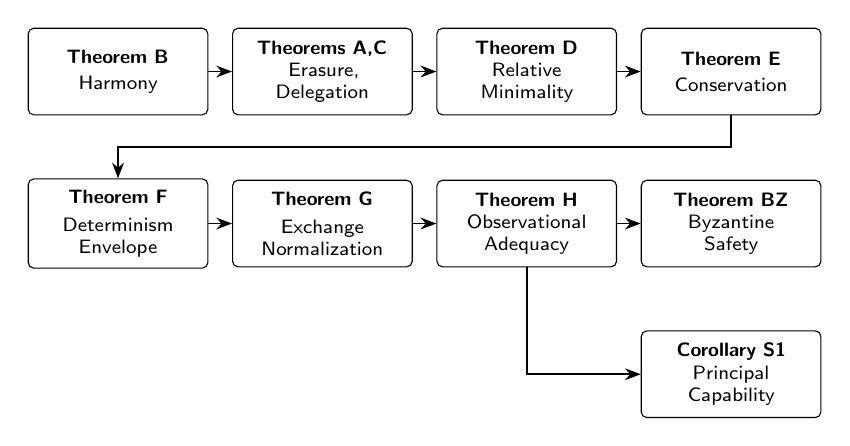
\begin{tikzpicture}[figfont, node distance=3mm]
				\def\depboxw{20mm}
				% Main dependency nodes - row 1
				\node[figsubbox, text width=\depboxw, minimum height=11mm] (B)
				{\vspace{-0.3ex}\textbf{Theorem B}\\[0.8ex]Harmony};
				\node[figsubbox, right=3mm of B, text width=\depboxw, minimum height=11mm] (AC)
				{\textbf{Theorems A,C}\\Erasure,\\Delegation};
				\node[figsubbox, right=3mm of AC, text width=\depboxw, minimum height=11mm] (D)
				{\textbf{Theorem D}\\Relative\\Minimality};
				\node[figsubbox, right=3mm of D, text width=\depboxw, minimum height=11mm] (E)
				{\vspace{-0.3ex}\textbf{Theorem E}\\[0.8ex]Conservation};

				% Main dependency nodes - row 2
				\node[figsubbox, below=8mm of B, text width=\depboxw, minimum height=11mm] (F)
				{\textbf{Theorem F}\\[2pt]Determinism\\Envelope};
				\node[figsubbox, right=3mm of F, text width=\depboxw, minimum height=11mm] (G)
				{\textbf{Theorem G}\\[2pt]Exchange\\Normalization};
				\node[figsubbox, right=3mm of G, text width=\depboxw, minimum height=11mm] (H)
				{\textbf{Theorem H}\\Observational\\Adequacy};
				\node[figsubbox, right=3mm of H, text width=\depboxw, minimum height=11mm] (BZ)
				{\textbf{Theorem BZ}\\Byzantine\\Safety};

				% Branch node row
				\node[figsubbox, below=8mm of BZ, text width=\depboxw, minimum height=11mm] (S1)
				{\textbf{Corollary S1}\\Principal\\Capability};

			% Main dependency arrows
			\draw[figarrowstrong] (B) -- (AC);
			\draw[figarrowstrong] (AC) -- (D);
				\draw[figarrowstrong] (D) -- (E);
					\coordinate (EFmid) at ($(E.south)!0.5!(F.north)$);
					\draw[figarrowstrong] (E.south) -- (E.south |- EFmid) -- (F.north |- EFmid) -- (F.north);
				\draw[figarrowstrong] (F) -- (G);
				\draw[figarrowstrong] (G) -- (H);
				\draw[figarrowstrong] (H) -- (BZ);
					\draw[figarrowstrong] (H.south) -- ++(0,-2mm) |- (S1.west);
				\end{tikzpicture}
			}%
		\caption{Theorem dependency graph}
		\label{fig:p3-dependency-graph}
\end{figure}

\begin{proposition}[Regime Monotonicity]
	If a theorem requires regime $R$, then any stronger regime $R'$ with $R \preceq R'$ preserves theorem validity.
\end{proposition}

\begin{proof}[Proof sketch]
	Assume $R \preceq R'$, so $\mathrm{Prem}(R) \subseteq \mathrm{Prem}(R')$ by definition. Any derivation under $R$ uses only premises from $\mathrm{Prem}(R)$, hence all of its premises are available under $R'$. Therefore theorem validity is monotone along the regime order.
\end{proof}

\subsection{Consequence of the Dependency Graph}

Structural theorems (A--D) are insensitive to quantitative profile constants; quantitative and envelope/byzantine claims are regime-indexed exactly as declared in main text assumption blocks.

\section{Deferred Transport Schemas}
\label{app:transport}

Transport results in Section~\ref{sec:transport} factor into structural and analytic layers.

\subsection{Generic Transport Rule}

\begin{theorem}[Transport by Premise Separation]
	\label{thm:app-p3-transport-separation}
	If structural premises of \ABHStack\ hold and analytic package $A_T$ holds for target claim $T$, then $T$ follows without strengthening structural premises.
\end{theorem}

\begin{proof}[Proof sketch]
	Map the structural side of \ABHStack\ into the interface required by $A_T$. Apply the analytic theorem in that interface to obtain the target claim. Then transport the conclusion back to the protocol statement through the same interface map. No extra semantic premise is added during transport.
\end{proof}

\subsection{Interface Discipline}

Transport statements must expose only:
\begin{enumerate}
	\item structural interface obligations (coherence/harmony/envelope/adherence),
	\item analytic assumptions external to this manuscript,
	\item resulting transported consequence.
\end{enumerate}

This prevents hidden strengthening of either side.

\subsection{Representative Schemas}

\begin{enumerate}
	\item Tail-bound transport schema:
	      \begin{equation}
		      \begin{aligned}
			      \text{Struct}_{B..H} \land \text{ConcentrationPkg}(\theta)
			       & \Longrightarrow                     \\
			      \forall t \ge 0,\ \Pr[X - \mathbb{E}X \ge t]
			       & \le \Psi_{\mathrm{tail}}(t;\theta).
		      \end{aligned}
	      \end{equation}
	\item Mixing/convergence transport schema:
	      \begin{equation}
		      \begin{aligned}
			      \text{Struct}_{B..H} \land \text{MixPkg}(\eta)
			       & \Longrightarrow                  \\
			      \forall n \ge 0,\ \|\mu_n - \mu_*\|_{\mathrm{TV}}
			       & \le \Psi_{\mathrm{mix}}(n;\eta).
		      \end{aligned}
	      \end{equation}
	\item Compositional exactness transport schema:
	      \begin{equation}
		      \begin{aligned}
			      \text{Struct}_{B..H} \land \text{NonInterference}
			       & \Longrightarrow \\
			      \EnvelopeExact(C_1) \land \EnvelopeExact(C_2)
			       & \Rightarrow     \\
			      \EnvelopeExact(C_1 \otimes C_2).
		      \end{aligned}
	      \end{equation}
	\item Byzantine adherence transport schema:
	      \begin{equation}
		      \begin{aligned}
			      \text{Struct}_{B..H}
			       & \land \text{ABlockD}      \\
			       & \land \text{WitnessPkg}   \\
			       & \Longrightarrow           \\
			      \mathsf{VMByzAdheres}
			       &                           \\
			       & \land \EqsafeConformance.
		      \end{aligned}
	      \end{equation}
\end{enumerate}

\section{Deferred Consequence Statements}
\label{app:consequences}

\subsection{Reconfiguration and Minimality}

\begin{proposition}
	Under Assumption Block~\ref{assump:p3-reconfiguration}, Harmony (Theorem~\ref{thm:harmony}) and Relative Minimality (Theorem~\ref{thm:minimality}) imply that any admissible safe-reconfiguration invariant implies $\Coherent$ and therefore factors through the same canonical safety core.
\end{proposition}

\begin{proof}[Proof sketch]
	Theorem~\ref{thm:minimality} shows that every admissible invariant factors through $\Coherent$. Theorem~\ref{thm:harmony} then gives commutation of reconfiguration steps over that common core. Chaining these two implications yields the proposition.
\end{proof}

\subsection{Envelope and Determinism Boundary}

\begin{proposition}
	Under Assumption Block~\ref{assump:p3-envelope}, Theorem~\ref{thm:envelope} and Theorem~\ref{thm:normalization} jointly characterize determinism modulo exchange/spatial normalization and identify strict boundary witnesses for inadmissible envelope extensions.
\end{proposition}

\begin{proof}[Proof sketch]
	Apply Theorem~\ref{thm:envelope} to obtain exact envelope characterization via soundness, realizability, and maximality. Apply Theorem~\ref{thm:normalization} to identify the normalized observational equalities that hold inside that exact envelope. Combining both gives the claimed determinism boundary statement.
\end{proof}

\subsection{Runtime Adequacy and Admission}

\begin{proposition}
	Under Assumption Block~\ref{assump:p3-adequacy}, Theorem~\ref{thm:adequacy} plus Corollary~\ref{cor:principal} yields principal-capability admission completeness with explicit rejection diagnostics when premise evidence is missing.
\end{proposition}

\begin{proof}[Proof sketch]
	Theorem~\ref{thm:adequacy} yields adequacy and adherence under Assumption Block~\ref{assump:p3-adequacy}. Corollary~\ref{cor:principal} then refines this with principal-capability inference and admission completeness. Together they imply the proposition.
\end{proof}

\subsection{Byzantine Scope Boundary}

\begin{proposition}
	Under Assumption Block~\ref{assump:p3-byzantine}, Theorem~\ref{thm:byzantine} and Corollary~\ref{cor:byzantine-converse} establish exact safety characterization and converse counterexample packaging, but do not establish Byzantine liveness outside declared timing/fairness assumptions.
\end{proposition}

\begin{proof}[Proof sketch]
	Theorem~\ref{thm:byzantine} and Corollary~\ref{cor:byzantine-converse} provide exact Byzantine safety characterization and converse counterexample packaging under Assumption Block~\ref{assump:p3-byzantine}. Section~\ref{sec:limitations} explicitly restricts scope away from weaker timing and fairness assumptions required for Byzantine liveness. Therefore the claimed boundary follows directly.
\end{proof}

\section{Mechanization Summary}
\label{app:mechanization}

Table~\ref{tab:p3-module-map} maps theorem families to concrete modules and theorem anchors.
Module references use path identifiers of the form \texttt{P$n$-A$xx$}, where $n$ is the paper number and $xx$ is the artifact index; these resolve to file paths in Appendix~\ref{app:p3-path-registry}.

\begin{table}[H]
	\centering
	\footnotesize
	\begin{tabularx}{\columnwidth}{@{}L{0.11\columnwidth}L{0.44\columnwidth}L{0.35\columnwidth}@{}}
		\toprule
		\thead{Thm} & \thead{Modules}                               & \thead{Anchors}                       \\
		\midrule
		B           & \pathref{P3-A08},\allowbreak \pathref{P3-A09} & \nolinkurl{link_harmony_through_link} \\
		A,C,D       & \pathref{P3-A10}                              & \nolinkurl{coherent_erasure_stable}   \\
			E           & \pathref{P3-A11},\allowbreak \pathref{P3-A12} & \nolinkurl{flagship_composed_system_conservation} \\
			F,G         & \pathref{P3-A13}                              & \nolinkurl{consensusEnvelope_exact_of_profile} \\
			H,S1        & \pathref{P3-A14},\allowbreak \pathref{P3-A15} & \nolinkurl{vm_adequacy_of_trace_consistency} \\
			BZ          & \pathref{P3-A16}                              & \nolinkurl{byzantineSafety_exact_of_profile} \\
		\bottomrule
	\end{tabularx}
	\caption{Module map.}
	\label{tab:p3-module-map}
\end{table}

\section{Artifact Path Registry}
\label{app:p3-path-registry}

All Lean file-path references in this paper use the identifiers listed in Table~\ref{tab:p3-path-registry}.

\begin{table}[H]
	\centering
	\footnotesize
	\begin{tabularx}{\columnwidth}{@{}L{0.2\columnwidth}L{0.75\columnwidth}@{}}
		\toprule
		\thead{ID}      & \thead{Path (relative to \texttt{lean/})}                          \\
		\midrule
		\texttt{P3-A01} & \texttt{Protocol/\allowbreak Coherence/\allowbreak}\mbox{\texttt{GraphDelta.lean}}                      \\
		\texttt{P3-A02} & \texttt{Protocol/\allowbreak Coherence/\allowbreak}\mbox{\texttt{GraphDeltaHO.lean}}                    \\
		\texttt{P3-A03} & \texttt{Protocol/\allowbreak Coherence/\allowbreak}\mbox{\texttt{ConfigEquiv.lean}}                     \\
		\texttt{P3-A04} & \texttt{Protocol/\allowbreak Coherence/\allowbreak ConfigEquivRenaming/\allowbreak}\mbox{\texttt{*.lean}}           \\
		\texttt{P3-A05} & \texttt{Protocol/\allowbreak Coherence/\allowbreak RoleSwap/\allowbreak}\mbox{\texttt{*.lean}}                      \\
		\texttt{P3-A06} & \texttt{Protocol/\allowbreak Coherence/\allowbreak Delegation/\allowbreak Core/\allowbreak}\mbox{\texttt{*.lean}}               \\
		\texttt{P3-A07} & \texttt{Protocol/\allowbreak Coherence/\allowbreak Delegation/\allowbreak}\mbox{\texttt{Preservation.lean}}         \\
		\texttt{P3-A08} & \texttt{Protocol/\allowbreak Deployment/\allowbreak}\mbox{\texttt{LinkingCore.lean}}                    \\
		\texttt{P3-A09} & \texttt{Runtime/\allowbreak Proofs/\allowbreak EffectBisim/\allowbreak}\mbox{\texttt{Congruence.lean}}              \\
		\texttt{P3-A10} & \texttt{Protocol/\allowbreak Coherence/\allowbreak}\mbox{\texttt{ErasureCharacterization.lean}}         \\
		\texttt{P3-A11} & \texttt{Protocol/\allowbreak Deployment/\allowbreak}\mbox{\texttt{LinkingTheorems.lean}}                \\
		\texttt{P3-A12} & \texttt{Runtime/\allowbreak Proofs/\allowbreak}\mbox{\texttt{Lyapunov.lean}}                            \\
		\texttt{P3-A13} & \texttt{Runtime/\allowbreak Adequacy/\allowbreak EnvelopeCore/\allowbreak}\mbox{\texttt{*.lean}}                    \\
		\texttt{P3-A14} & \texttt{Runtime/\allowbreak Adequacy/\allowbreak}\mbox{\texttt{Adequacy.lean}}                          \\
		\texttt{P3-A15} & \texttt{Runtime/\allowbreak Proofs/\allowbreak TheoremPack/\allowbreak}\mbox{\texttt{*.lean}}                       \\
		\texttt{P3-A16} & \texttt{Runtime/\allowbreak Proofs/\allowbreak Adapters/\allowbreak Distributed/\allowbreak}\mbox{\texttt{EnvelopeTheorems.lean}} \\
		\bottomrule
	\end{tabularx}
	\caption{Artifact path registry for \emph{Harmony from Coherence in Asynchronous MPST}.}
	\label{tab:p3-path-registry}
\end{table}

\section{Reproducibility}
\label{app:reproducibility}

Reproduction uses the pinned Lean toolchain and manifest.

\begin{enumerate}
	\item Build theorem families listed in Table~\ref{tab:p3-module-map}.
	\item Run \texttt{just escape} and \texttt{just verify-protocols}.
	\item Validate that Table~\ref{tab:p3-module-map} anchor names resolve and no proof holes remain.
\end{enumerate}

Expected outcome: Full theorem-dependency compilation for Theorems~\ref{thm:harmony}--\ref{thm:adequacy}, Corollary~\ref{cor:principal}, Theorem~\ref{thm:byzantine}, and Corollary~\ref{cor:byzantine-converse} succeeds, profile extraction and admission modules compile, and bridge and adequacy modules compile under the pinned toolchain.

\section{Index of Main Results}
\label{app:index}

\begin{table}[H]
	\centering
	\footnotesize
	{\setlength{\tabcolsep}{3pt}
	\begin{tabularx}{\columnwidth}{@{}L{0.22\columnwidth}L{0.09\columnwidth}L{0.32\columnwidth}L{0.27\columnwidth}@{}}
		\toprule
		\thead{Claim}          & \thead{Sec.} & \thead{Assumptions}                   & \thead{Location}        \\
		\midrule
		Thm.~\ref{thm:harmony}            & \S\ref{sec:theorem-b} & Assump.~\ref{assump:p3-reconfiguration} & \pathref{P3-A08}, \pathref{P3-A09} \\
		Thm.~\ref{thm:erasure}            & \S\ref{sec:theorem-a} & Assump.~\ref{assump:p3-core}            & \pathref{P3-A10}                    \\
		Thm.~\ref{thm:delegation}         & \S\ref{sec:theorem-c} & Assump.~\ref{assump:p3-reconfiguration} & \pathref{P3-A10}                    \\
		Cor.~\ref{cor:footprint}          & \S\ref{sec:theorem-c} & Thm.~\ref{thm:delegation} + side conds  & \pathref{P3-A10}                    \\
		Thm.~\ref{thm:minimality}         & \S\ref{sec:theorem-d} & admissibility clauses + core model       & \pathref{P3-A10}                    \\
		Thm.~\ref{thm:conservation}       & \S\ref{sec:theorem-e} & Assump.~\ref{assump:p3-reconfiguration} + quant.\ profile & \pathref{P3-A11}, \pathref{P3-A12} \\
		Cor.~\ref{cor:compositional}      & \S\ref{sec:theorem-e} & non-interference + envelope exactness    & \S\ref{sec:theorem-e}               \\
		Thm.~\ref{thm:envelope}           & \S\ref{sec:theorem-f} & Assump.~\ref{assump:p3-envelope}         & \pathref{P3-A13}                    \\
		Cor.~\ref{cor:transportability}   & \S\ref{sec:theorem-f} & Assump.~\ref{assump:p3-envelope}         & \pathref{P3-A13}                    \\
		Cor.~\ref{cor:boundary}           & \S\ref{sec:theorem-f} & Assump.~\ref{assump:p3-envelope}         & \pathref{P3-A13}                    \\
		Cor.~\ref{cor:embedding}          & \S\ref{sec:theorem-f} & Assump.~\ref{assump:p3-envelope}         & \pathref{P3-A13}                    \\
		Thm.~\ref{thm:normalization}      & \S\ref{sec:theorem-g} & Assump.~\ref{assump:p3-envelope} + exch./spatial premises & \pathref{P3-A13} \\
		Thm.~\ref{thm:adequacy}           & \S\ref{sec:theorem-h} & Assump.~\ref{assump:p3-adequacy}         & \pathref{P3-A14}, \pathref{P3-A15} \\
		Prop.~\ref{prop:capability}       & \S\ref{sec:theorem-h} & Assump.~\ref{assump:p3-adequacy}         & \pathref{P3-A15}                    \\
		Cor.~\ref{cor:principal}          & \S\ref{sec:theorem-h} & adequacy + admission premises            & \pathref{P3-A15}                    \\
		Thm.~\ref{thm:byzantine}          & \S\ref{sec:theorem-h} & Assump.~\ref{assump:p3-byzantine}        & \pathref{P3-A16}                    \\
		Cor.~\ref{cor:byzantine-converse} & \S\ref{sec:theorem-h} & Thm.~\ref{thm:byzantine} + dropped class & \pathref{P3-A16}                    \\
		Prop.~\ref{prop:byzantine-vm}     & \S\ref{sec:theorem-h} & adequacy + Byzantine profile + capability bits & \pathref{P3-A15}, \pathref{P3-A16} \\
		Thm.~\ref{thm:tail}               & \S\ref{sec:transport} & Assump.~\ref{assump:p3-transport}        & \S\ref{sec:transport}               \\
		Thm.~\ref{thm:mixing}             & \S\ref{sec:transport} & Assump.~\ref{assump:p3-transport}        & \S\ref{sec:transport}               \\
		\bottomrule
	\end{tabularx}
	}
	\caption{Index of main results.}
	\label{tab:p3-index}
\end{table}

\end{document}
